\subsubsection{Generic contracts}
\paragraph{Security contracts}
\subparagraph{Owned}
This contract defines the owner of a contract. In Soldino the owner is the address which deploy all contracts. The contract defines a modifier, \texttt{onlyOwner}, used to allow only the owner to call a function which uses 
the above-mentioned modifier.
\begin{figure}[H]
	\centering
	\frame{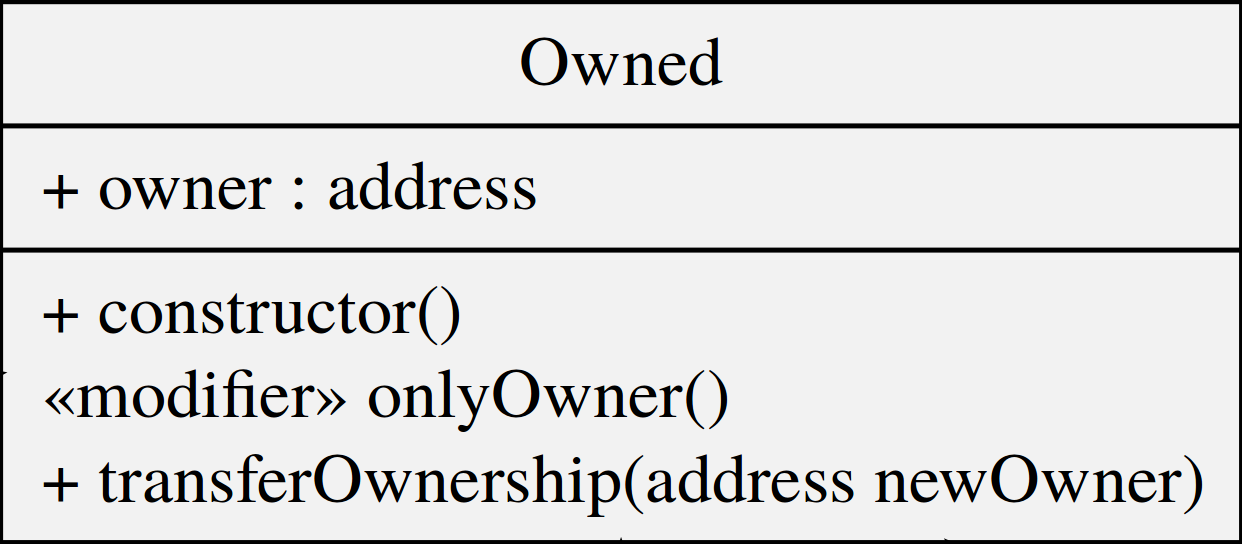
\includegraphics[scale=0.132]{res/images/solidity/owned.png}}
	\caption{class diagram of the Owned contract}
\end{figure}

\subparagraph{Authorizable}
This contract is used by all storage contracts. It's a derivate contract of \texttt{Owned} and stores 
all the addresses authorized to call the functions that use the modifier \texttt{onlyAuthorized} defined in this contract.
To authorize a contract the owner needs to call the function \texttt{addAuthorized}.
\begin{figure}[H]
	\centering
	\frame{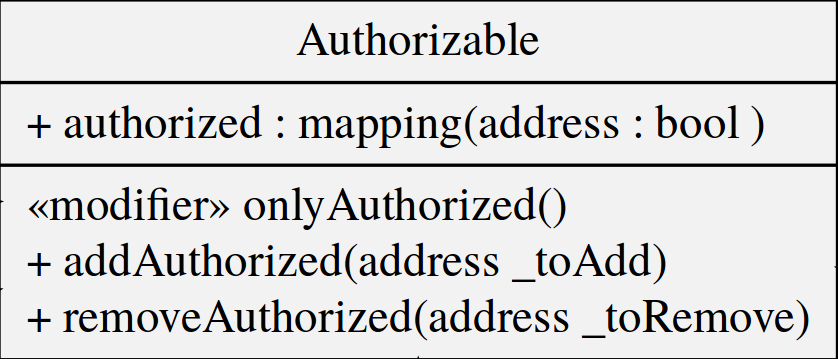
\includegraphics[scale=0.2]{res/images/solidity/authorizable.png}}
	\caption{class diagram of the Authorizable contract}
\end{figure}
\pagebreak
\paragraph{Token ERC20}\mbox{}\\

\noindent The contract \texttt{TokenCubit} implements the custom token \textit{Cubit}, stores all the users' balances and defines all the methods in order to be ERC20 compliant.
\begin{figure}[H]
	\centering
	\frame{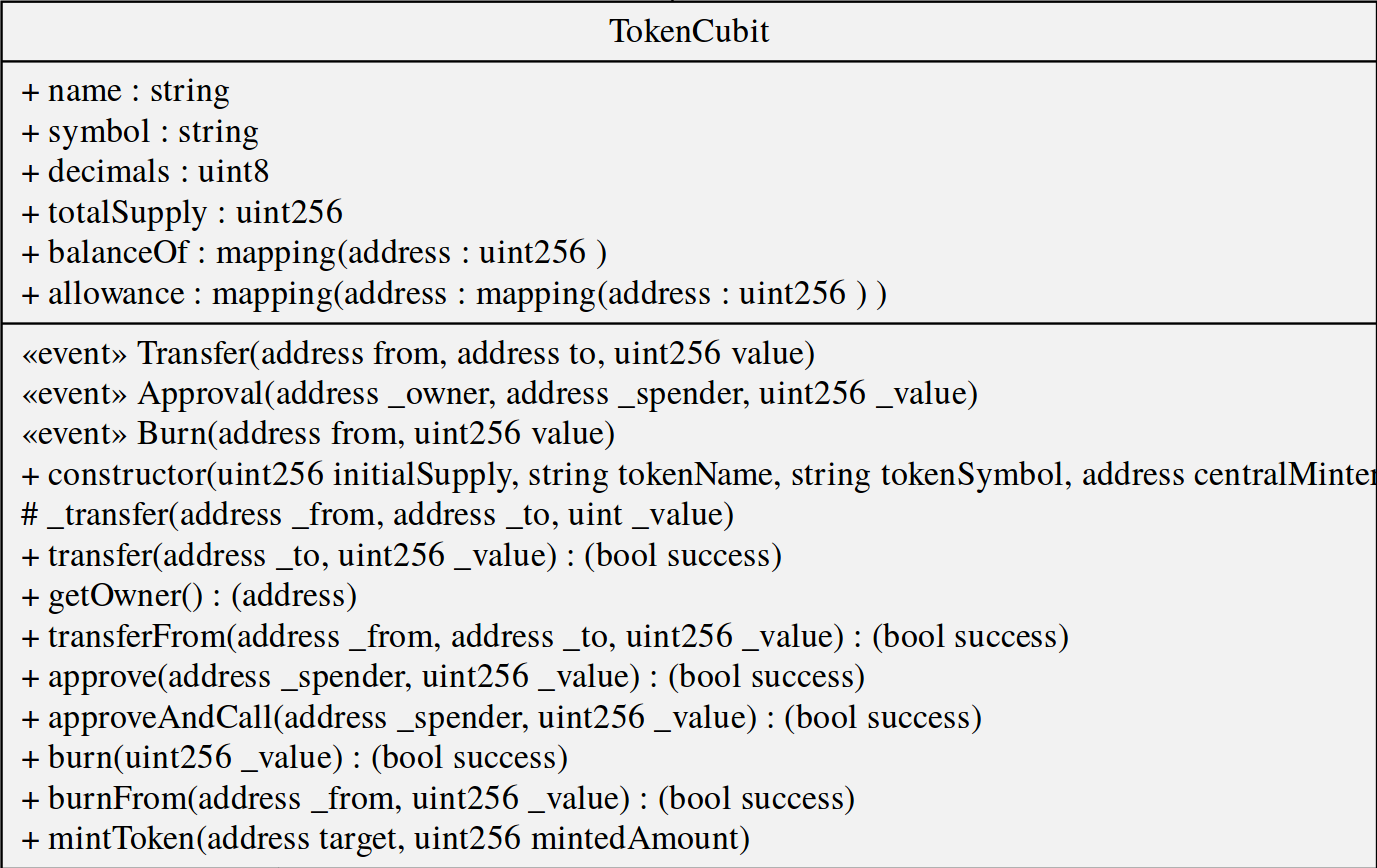
\includegraphics[scale=0.25]{res/images/solidity/tokencubit.png}}
	\caption{class diagram of the TokenCubit contract}
\end{figure}

\paragraph{ContractManager}\mbox{}\\ 

\noindent The purpose of the \texttt{ContractManager} is to achieve simple and cost effective upgradeability of the logic contracts. This contract stores a map in which the entries are composed in the following way:
\begin{itemize}
	\item\textbf{Key}: the contract name;
	\item\textbf{Value}: the last version of the contract deployment address.
\end{itemize}
When contract $A$ needs to communicate with another contract $B$, contract $A$ get the address of the last version of the contract $B$ from \texttt{ContractManager}. In this way there's no need to manage all the references in the contracts. 
\begin{figure}[H]
	\centering
	\frame{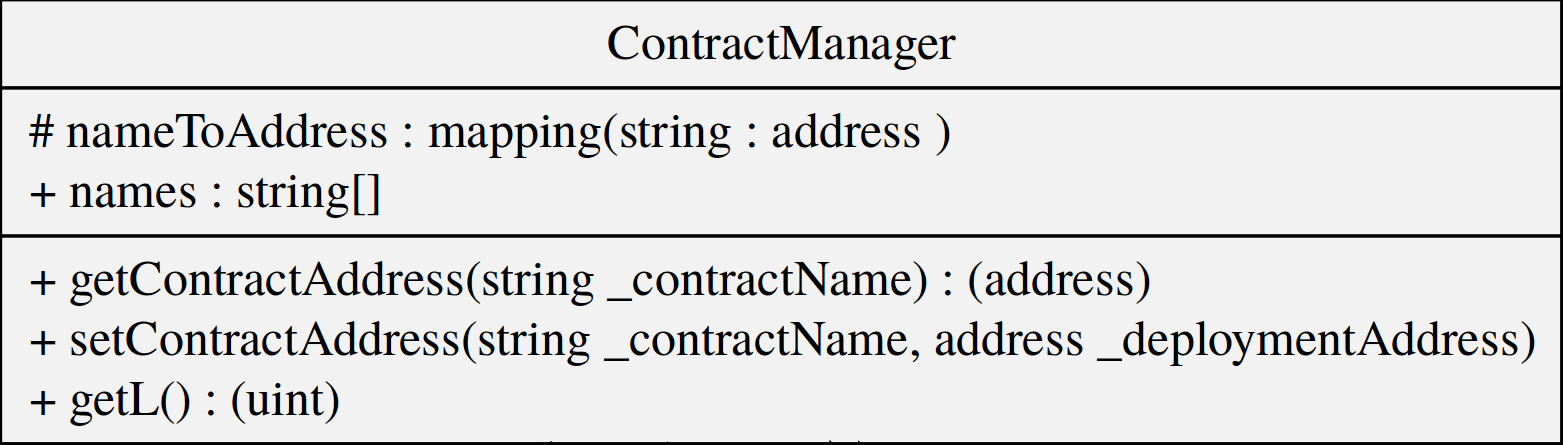
\includegraphics[scale=0.2]{res/images/solidity/contractmanager.png}}
	\caption{class diagram of the ContractManager contract}
\end{figure}
\pagebreak
\paragraph{Purchase}\mbox{}\\ 

\noindent The \texttt{Purchase} contract acts as a façade when it comes to buy products on Soldino.
Usually the user needs to confirm $n$ transactions for each order (intended as one order for each seller) to buy all the products in his cart, where $n$ is the number of orders.\\
With the \texttt{Purchase} contract, the user has to confirm always two transactions, no matter how many products are in his cart. 
\begin{figure}[H]
	\centering
	\frame{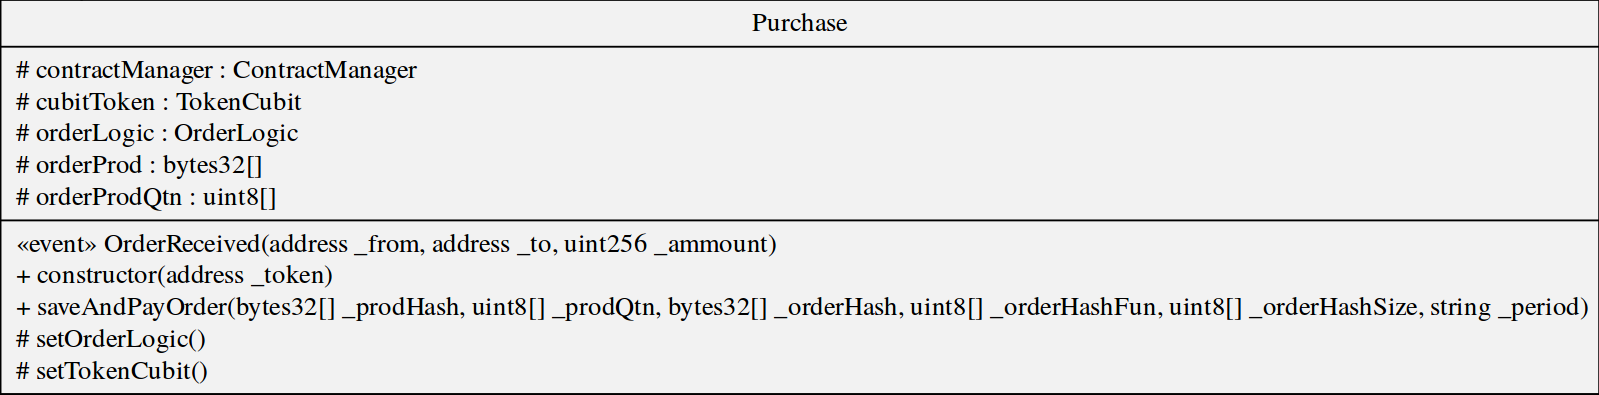
\includegraphics[scale=0.25]{res/images/solidity/purchase.png}}
	\caption{class diagram of the Purchase contract}
\end{figure}